%%%%%%%%%%%%%%%%%%%%%%%%%%%%%%%%%%%%%%%%%
% Focus Beamer Presentation
% LaTeX Template
% Version 1.0 (8/8/18)
%
% This template has been downloaded from:
% http://www.LaTeXTemplates.com
%
% Original author:
% Pasquale Africa (https://github.com/elauksap/focus-beamertheme) with modifications by 
% Vel (vel@LaTeXTemplates.com)
%
% Template license:
% GNU GPL v3.0 License
%
% Important note:
% The bibliography/references need to be compiled with bibtex.
%
%%%%%%%%%%%%%%%%%%%%%%%%%%%%%%%%%%%%%%%%%
%----------------------------------------------------------------------------------------
%	PACKAGES AND OTHER DOCUMENT CONFIGURATIONS
%----------------------------------------------------------------------------------------
\documentclass{beamer}
\usetheme[numbering=fullbar]{focus} % Use the Focus theme supplied with the template
% Add option [numbering=none] to disable the footer progress bar
% Add option [numbering=fullbar] to show the footer progress bar as always full with a slide count
% Uncomment to enable the ice-blue theme
%\definecolor{main}{RGB}{92, 138, 168}
%\definecolor{background}{RGB}{240, 247, 255}
%------------------------------------------------
\usepackage{booktabs} % Required for better table rules
\usepackage[utf8]{inputenc} % Set up input encoding for spanish
\usepackage[T1]{fontenc} % Set up font encoding for spanish
\usepackage[spanish, mexico]{babel} % Translation of environments
\usepackage{dirtytalk} % Allows double quotes with \say{text}
\usepackage{graphicx} % To insert images
\usepackage{siunitx} % Sistema internacional de unidades
\usepackage[version=4]{mhchem} % Ecuaciones químicas.
\usepackage{xcolor} % Da color a tu vida.
\usepackage{hyperref} % URLS
\hypersetup{
    colorlinks=true,
    linkcolor=blue,
    filecolor=magenta,      
    urlcolor=cyan,
}
\graphicspath{ {Images/}}
%----------------------------------------------------------------------------------------
%	 TITLE SLIDE
%----------------------------------------------------------------------------------------
\title{Efecto del pH en el daño por radiación en cristales de proteína}
%\subtitle{Subtitle}
\author{Francisco Murphy Pérez \\ Dr. Enrique Rudiño Piñera}
%\titlegraphic{
\includegraphics[scale=1.25]{Images/focuslogo.pdf}} % Optional title page image, comment this line to remove it
\institute{Instituto de Biotecnología \\ Universidad Nacional Autónoma de México}
\date{27 04 2020}
%----------------------------------------------------------------------------------------
\begin{document}
%----------------------------------------------------------------------------------------
\begin{frame}
	\maketitle % Automatically created using the information in the commands above
\end{frame}
%----------------------------------------------------------------------------------------
%	 INTRODUCCIÓN
%----------------------------------------------------------------------------------------
\section{Introducción}
%----------------------------------------------------------------------------------------
\begin{frame}{Cristalografía de rayos X}
Actualmente la cristalografía de rayos X (CRX), es el método principal para obtener la estructura de tu proteína favorita. De 163141 estructuras depositadas en la base de datos de proteínas (PDB)\footnote{\url{https://www.rcsb.org/}.}, 145083 se han determinado gracias a este método\footnote{A 25 de abril del 2020.}. Esto representa el \SI{88.93}{\percent} del total.
\end{frame}
%----------------------------------------------------------------------------------------
\begin{frame}{El experimento de CRX}
De manera muy somera, el experimento de CRX consiste en:
\begin{enumerate}
  \item Incidir \alert{rayos X} sobre el cristal de proteína. 
  \item Obtener el patrón de difracción. 
  \item Rotar el cristal en cierto eje. 
  \item Repetir los pasos anteriores $n$ veces.
\end{enumerate}
\end{frame}
%----------------------------------------------------------------------------------------
\begin{frame}{Fuentes de rayos X}
 La fuente de rayos X más común, es la radiación sincrotrón. De 145083 estructuras determinadas por la CRX, 114781 fueron determinadas en un sincrotrón\footnote{A 25 de abril del 2020}. Esto representa el \SI{79.11}{\percent}.
\end{frame}
%----------------------------------------------------------------------------------------
\begin{frame}{Daño por radiación}
Una de las limitantes de la CRX, es el daño por radiación que se clasifica según su componente temporal \cite{Teng2000}.
  \begin{enumerate}
	\item Daño primario (fotoionización)
	\item Daño secundario (cascada de radicales libres)
	\item Daño terciario (pérdida de la red cristalina)
	\end{enumerate}
\end{frame}
%----------------------------------------------------------------------------------------
% \begin{frame}
% \begin{figure}[h]
%   \centering
%   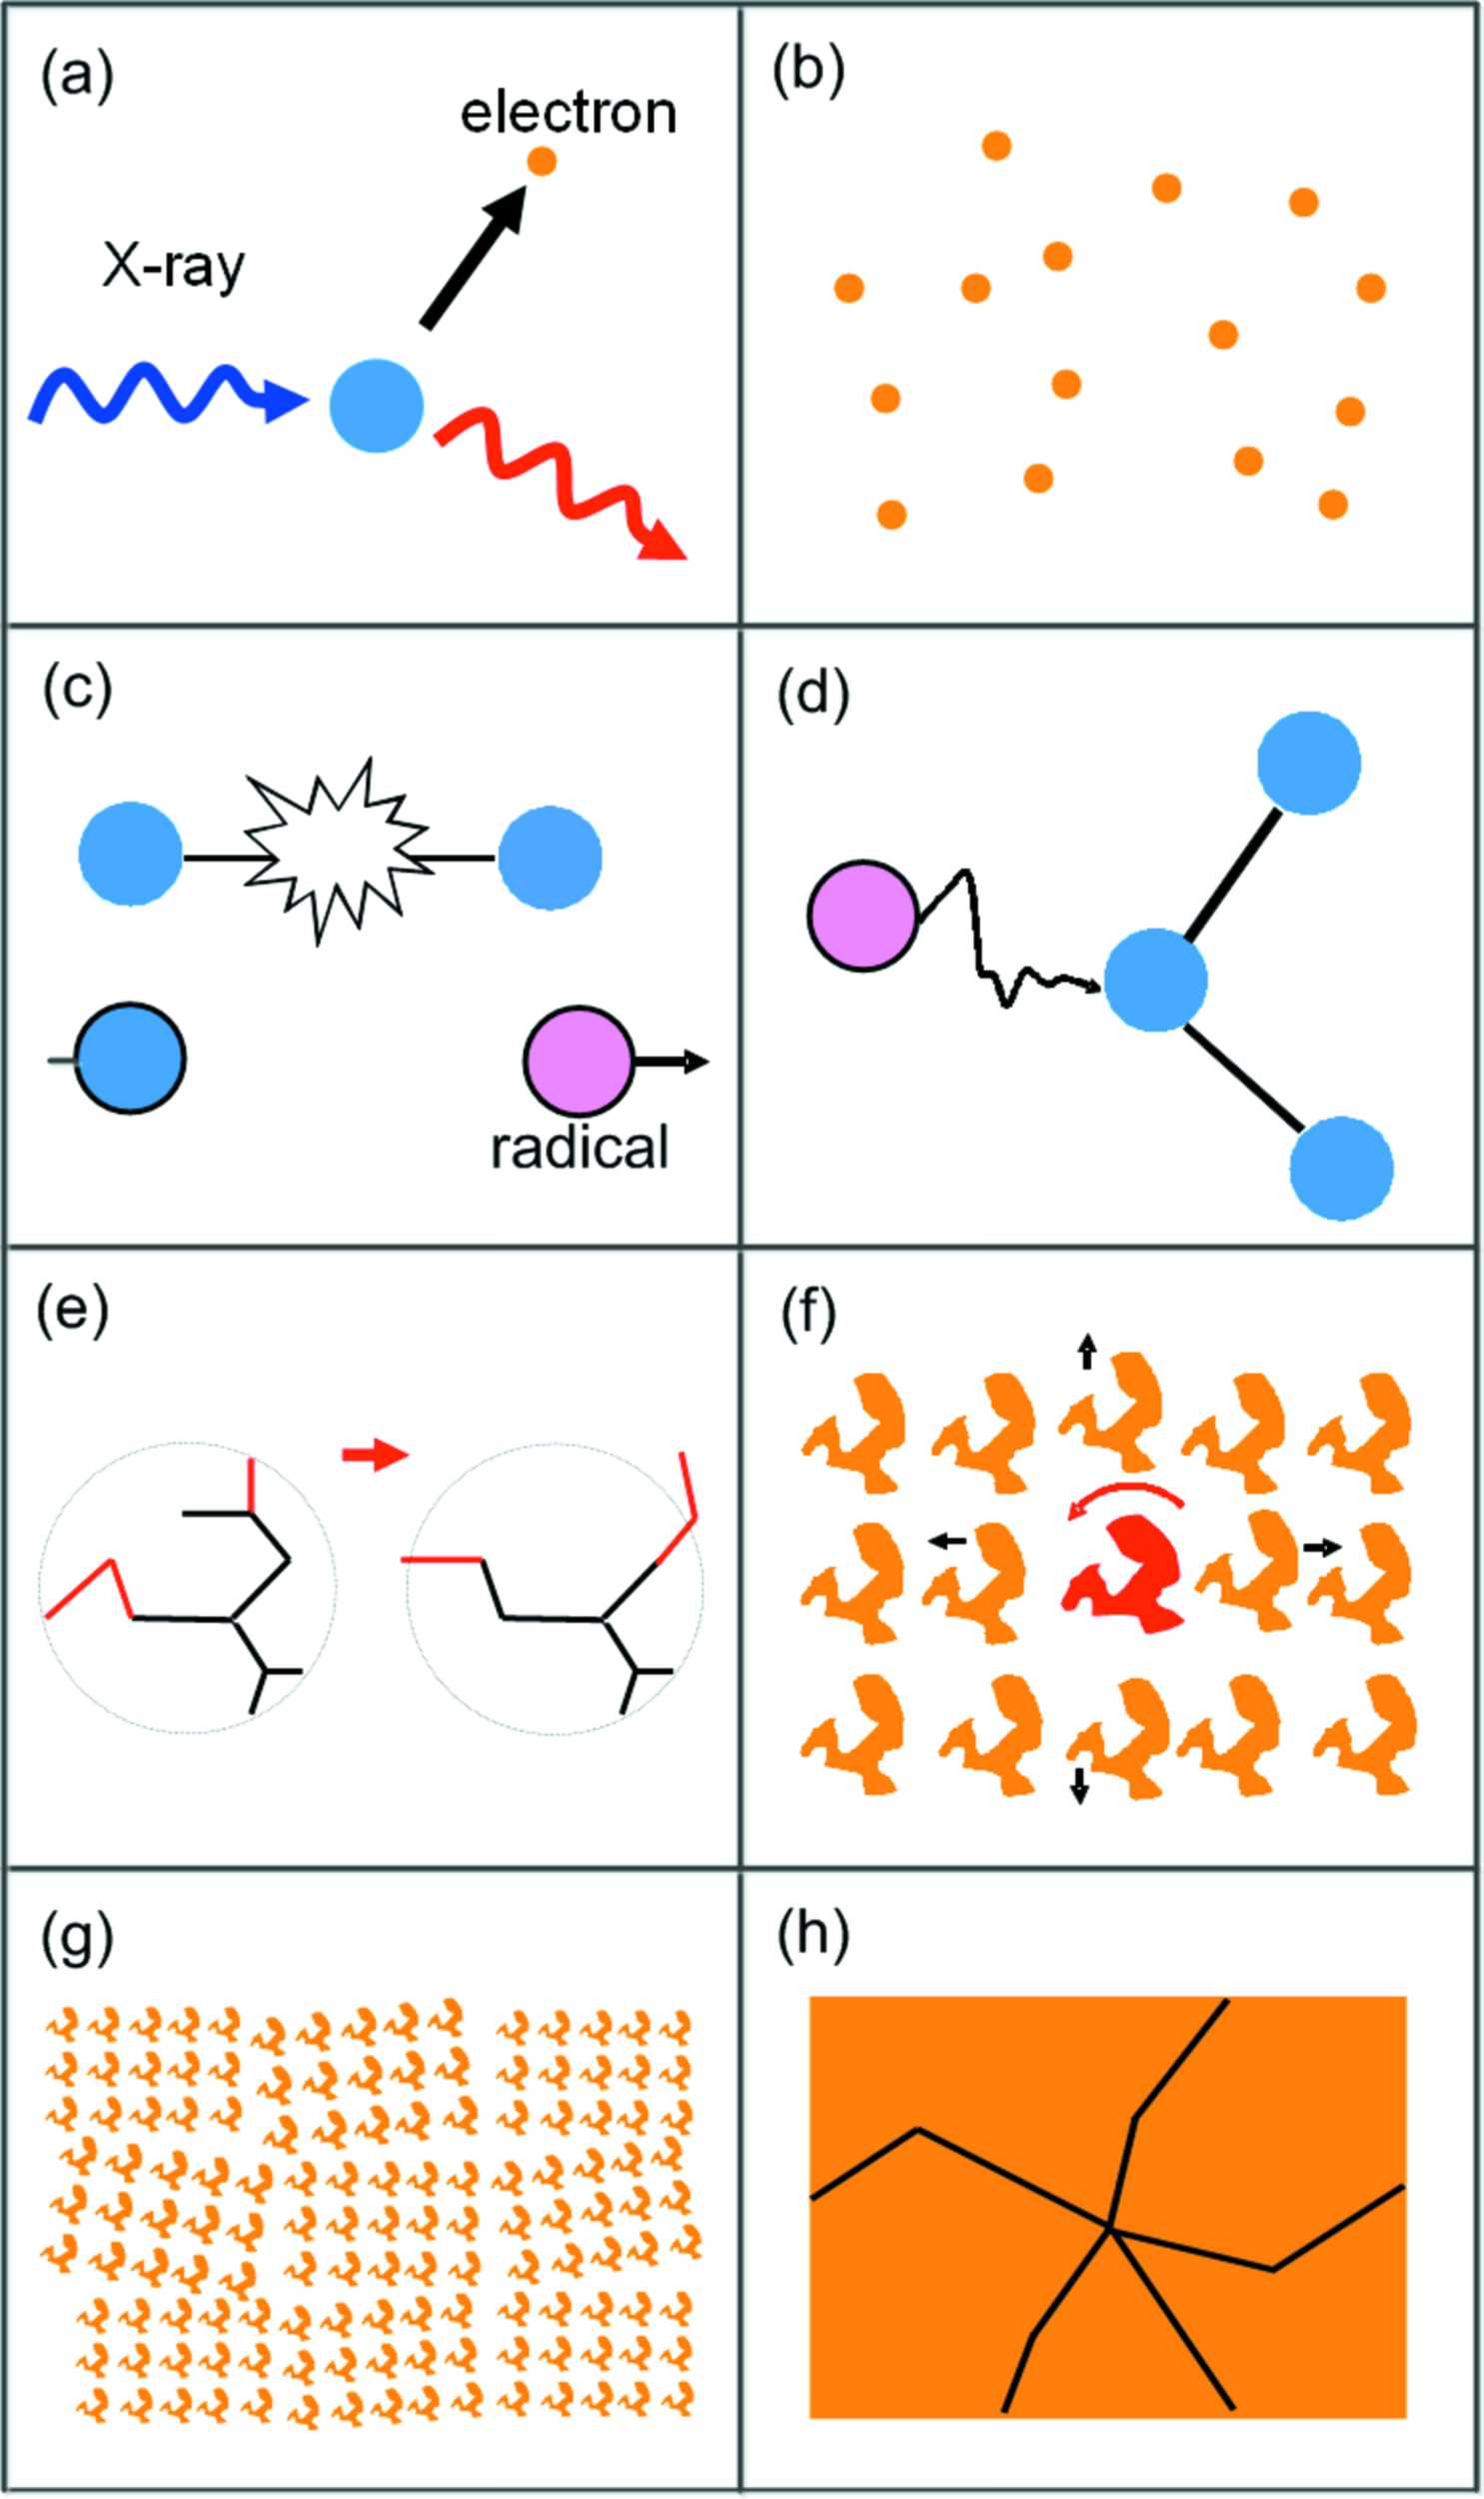
\includegraphics[width=0.8\textwidth]{warkentin.png}
%   \caption{Daño por radiación en cristales de proteína. Fuente: \cite{Warkentin2013}. }
%   \label{fig:warkentin2013}
% \end{figure}
% \end{frame}
%----------------------------------------------------------------------------------------
\begin{frame}{Daño primario}
\begin{figure}
  \begin{align}
  \ce{H2O           &->[rayos X]     H2O^{.+}    +             e^{-}}  \\
  \ce{H2O           &->[rayos X]     H2O^{*}}                          \\
  \ce{H2O^{.+}      &->  \color{red}HO^{.}       +              H^{+}} \\
  \ce{e^{-} + nH2O  &->  \color{red}e^{-}_{solv.}}                     \\
  \ce{H2O^{*}       &->  \color{red}HO^{.}       +   \color{red}H^{.}}
  \end{align} 
  \caption{Fotoionización de una molécula de agua y reacciones subsecuentes. Fuente: \cite{VonSonntag2006}.}  
  \label{fig:vonsonntag2006}
\end{figure}
\end{frame}
%----------------------------------------------------------------------------------------
\begin{frame}{Crioprotección}
Una de las primeras estrategias para minimizar el daño por radiación fue realizar el experimento de difracción a bajas temperaturas.
\begin{figure}[h]
	\centering
	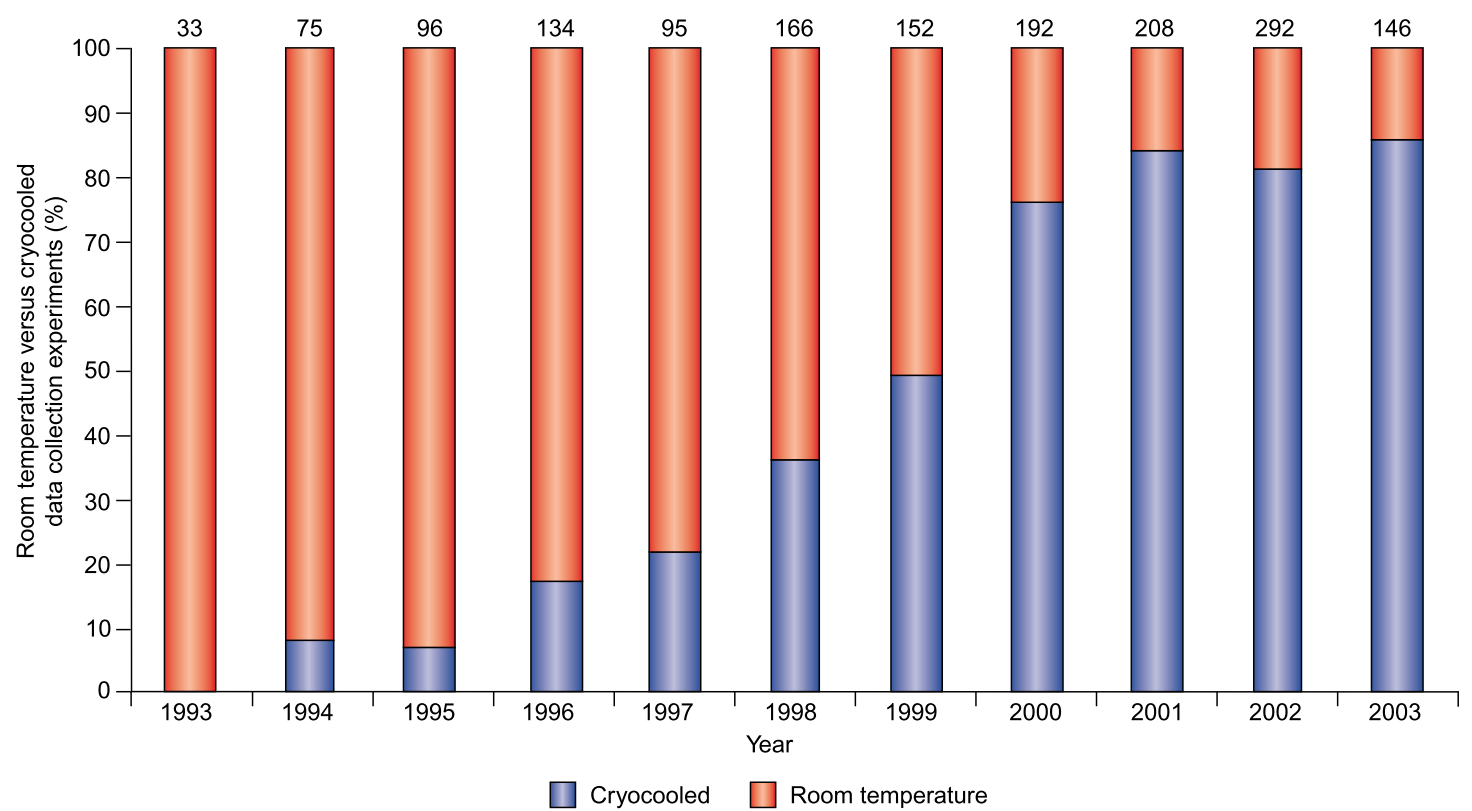
\includegraphics[width=0.8\textwidth]{garman2003.png}
	\caption{Adopción de la crioprotección. Imagen tomada de \cite{Garman2003}.}
	\label{fig:garman2003}
\end{figure}
\end{frame}
%----------------------------------------------------------------------------------------
\begin{frame}{Difusión de radicales}
\begin{figure}
  \begin{align*}
  \ce{H2O           &->[rayos X]     H2O^{.+}    +             e^{-}}  \\
  \ce{H2O           &->[rayos X]     H2O^{*}}                          \\
  \ce{H2O^{.+}      &->  \color{blue}HO^{.}       +              H^{+}} \\
  \ce{e^{-} + nH2O  &->  \color{red}e^{-}_{solv.}}                     \\
  \ce{H2O^{*}       &->  \color{blue}HO^{.}       +   \color{red}H^{.}}
  \end{align*} 
  \caption{Se impide la difusión de \ce{HO^{.}} (\SI{-173.15}{\celsius}). Fuente: \cite{Owen2012a}.}  
  \label{fig:owen2012a}
\end{figure}
\end{frame}
%----------------------------------------------------------------------------------------
\begin{frame}{Difusión de radicales}
El \ce{e^{-}_{solv.}} puede viajar a través de la cadena polipeptídica hasta encontrar un centro electrofílico. 
\begin{figure}[h]
  \centering
  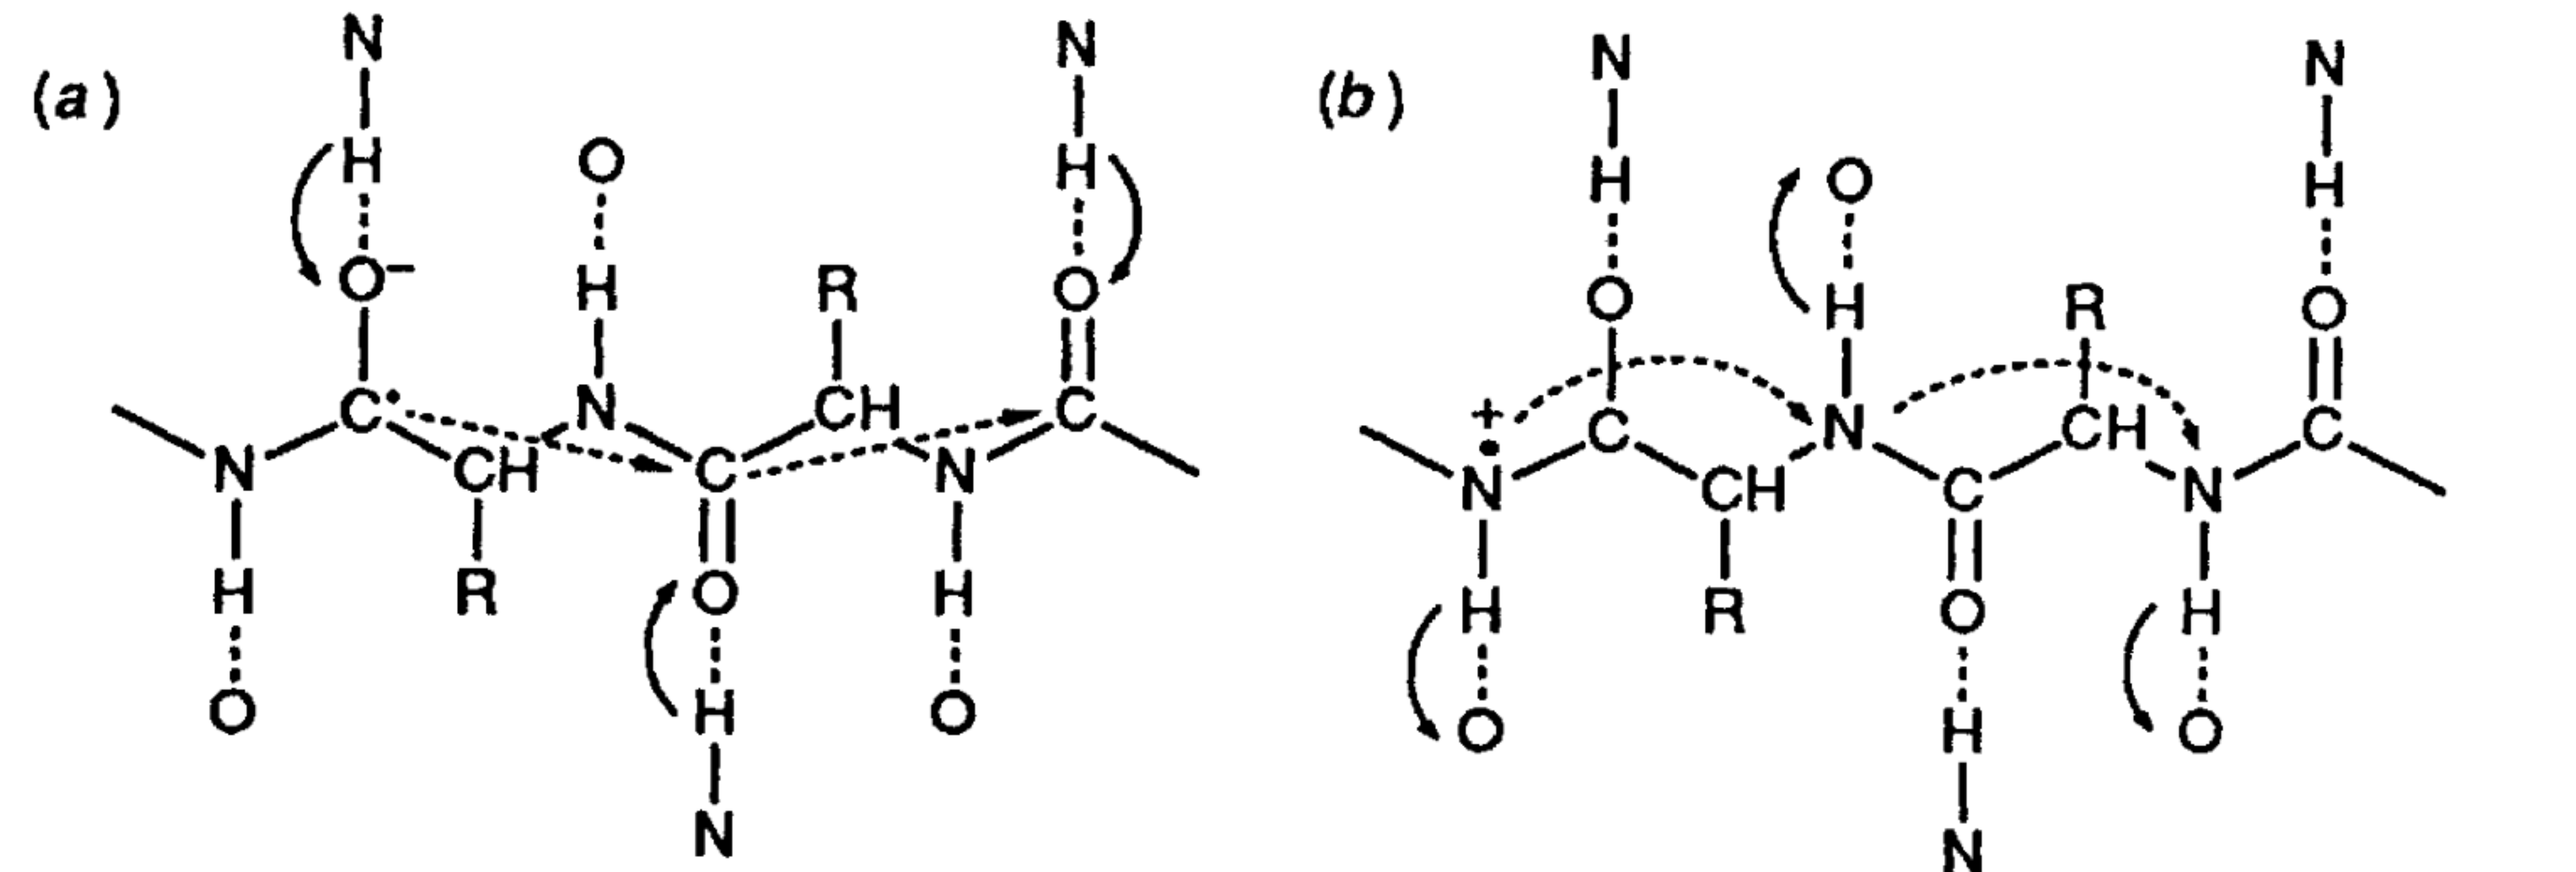
\includegraphics[width=0.7\textwidth]{symons92.png}
  \caption{Moviento de electrones (a) y huecos positivos (b), a través de la cadena polipeptídica. Fuente: \cite{Symons1992}}
  \label{fig:symons92}
\end{figure}
\end{frame}
%----------------------------------------------------------------------------------------
\begin{frame}{Consecuencias: daño específico}
  \begin{figure}[h]
    \centering
    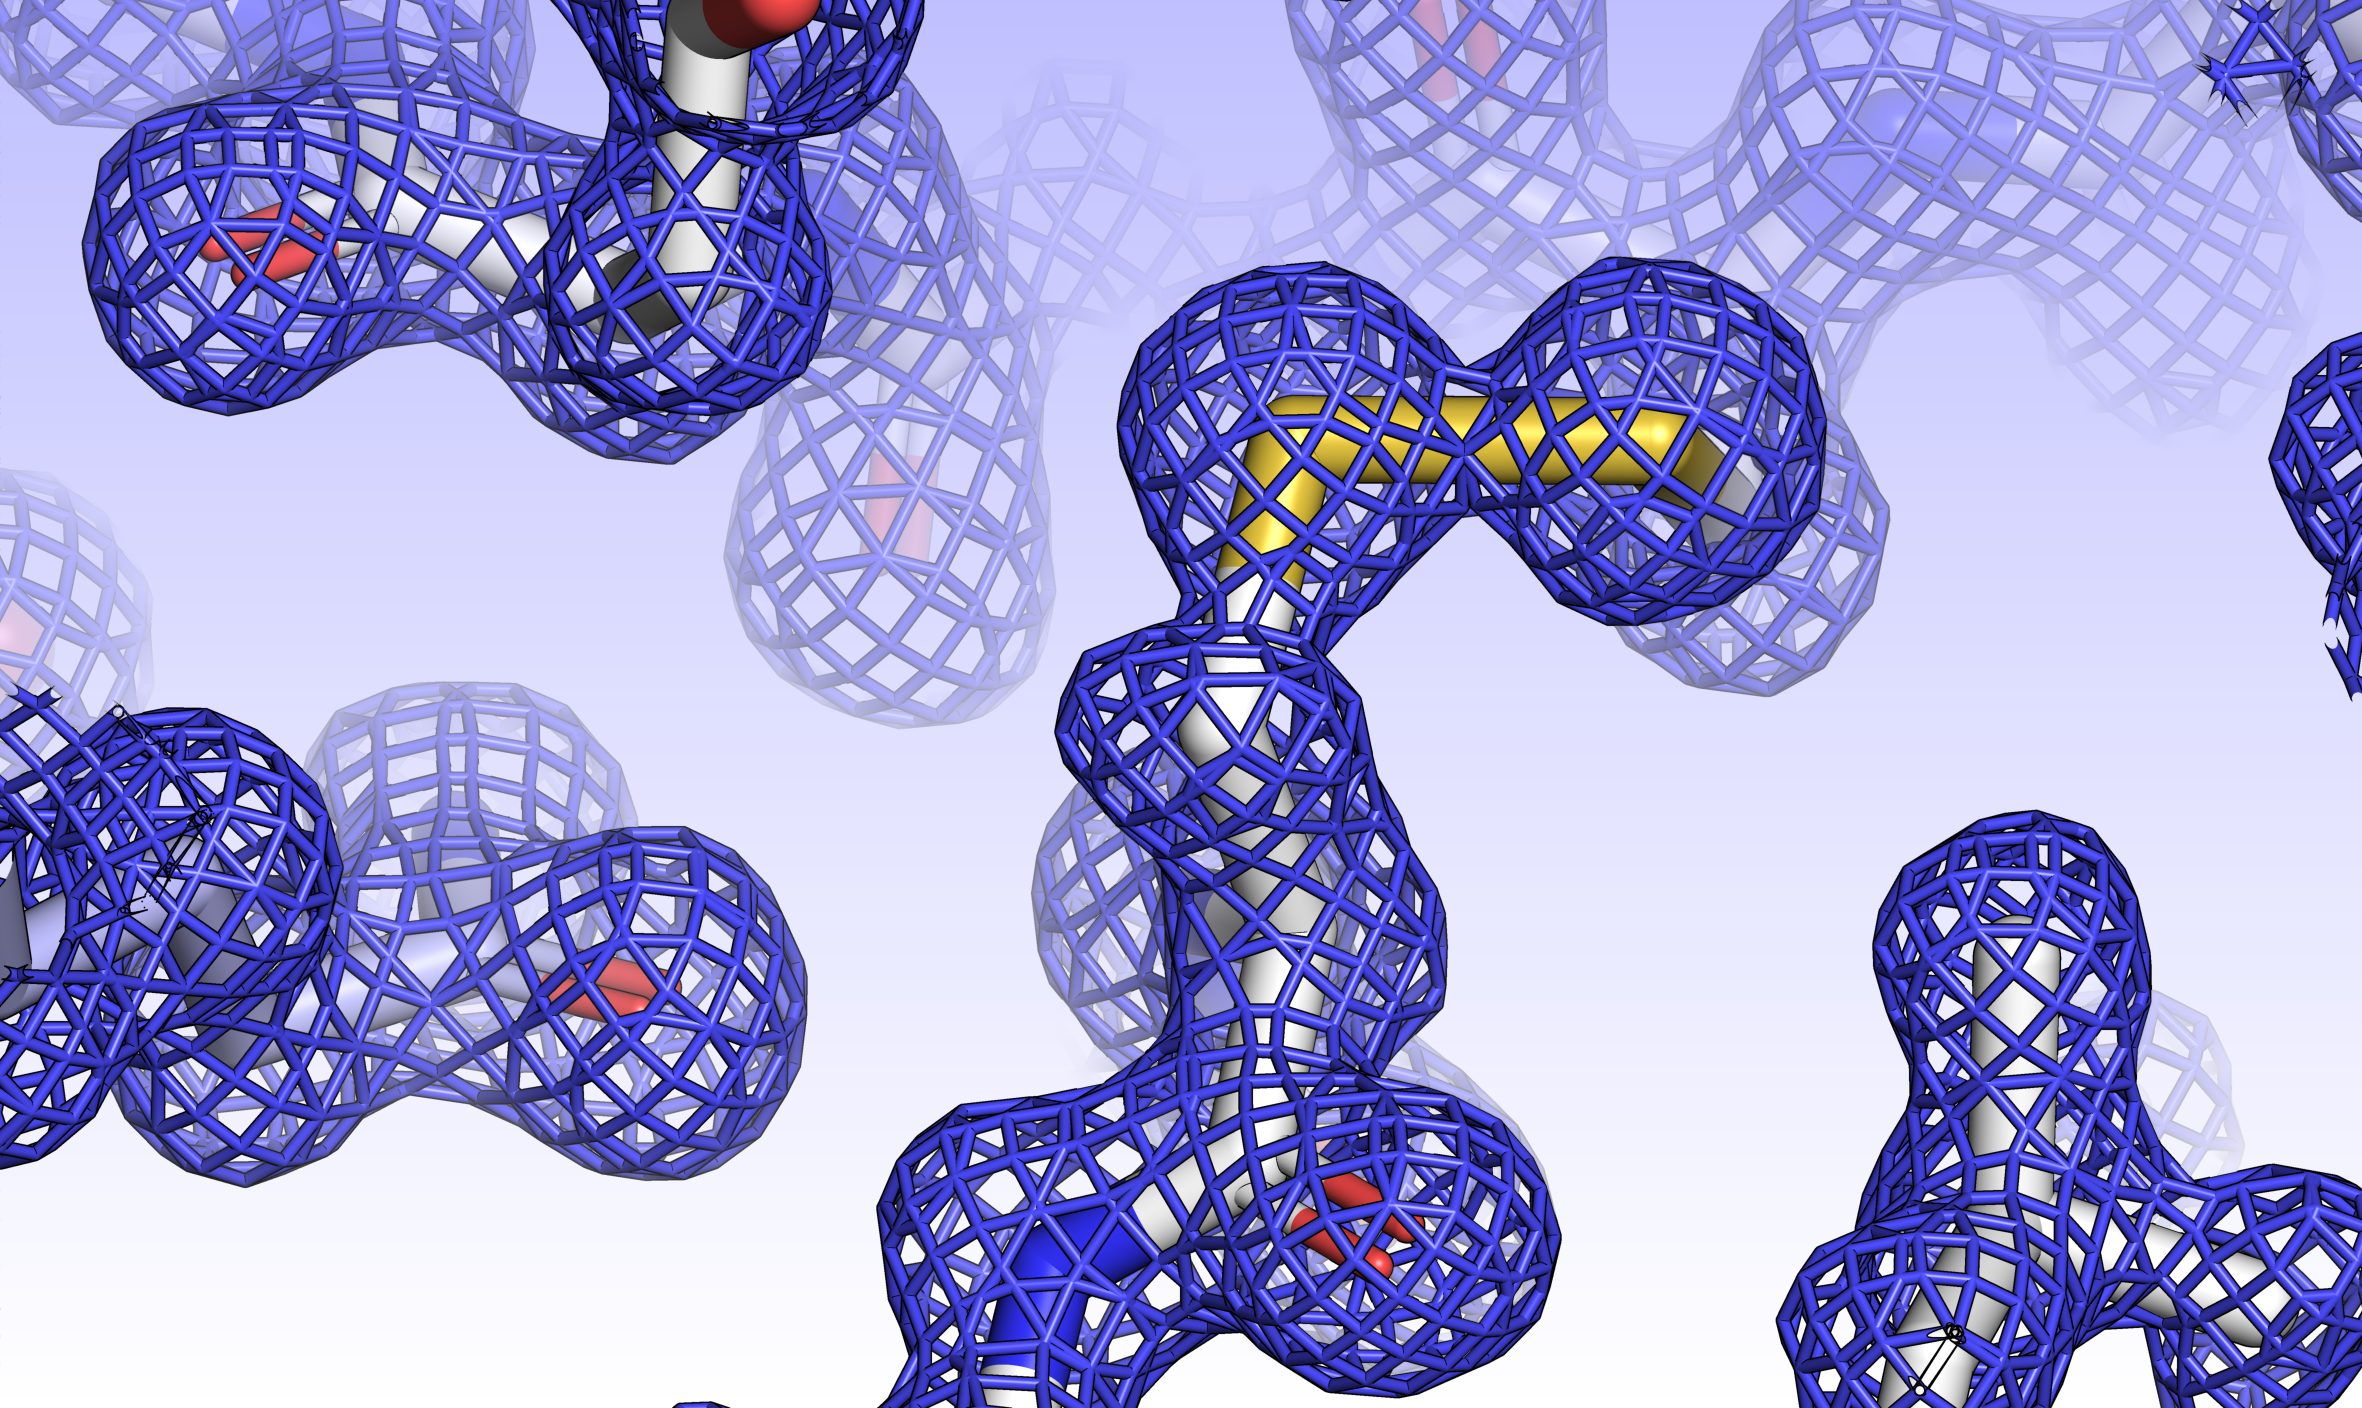
\includegraphics[width=0.8\textwidth]{before.png}
    \caption{Lisozima, colecta 1 a \SI{0.6}{\mega\gray}. Datos de \cite{Nanao2005}.}
  \end{figure}
\end{frame}
%----------------------------------------------------------------------------------------
\begin{frame}{Consecuencias: daño específico}
  \begin{figure}[h]
    \centering
    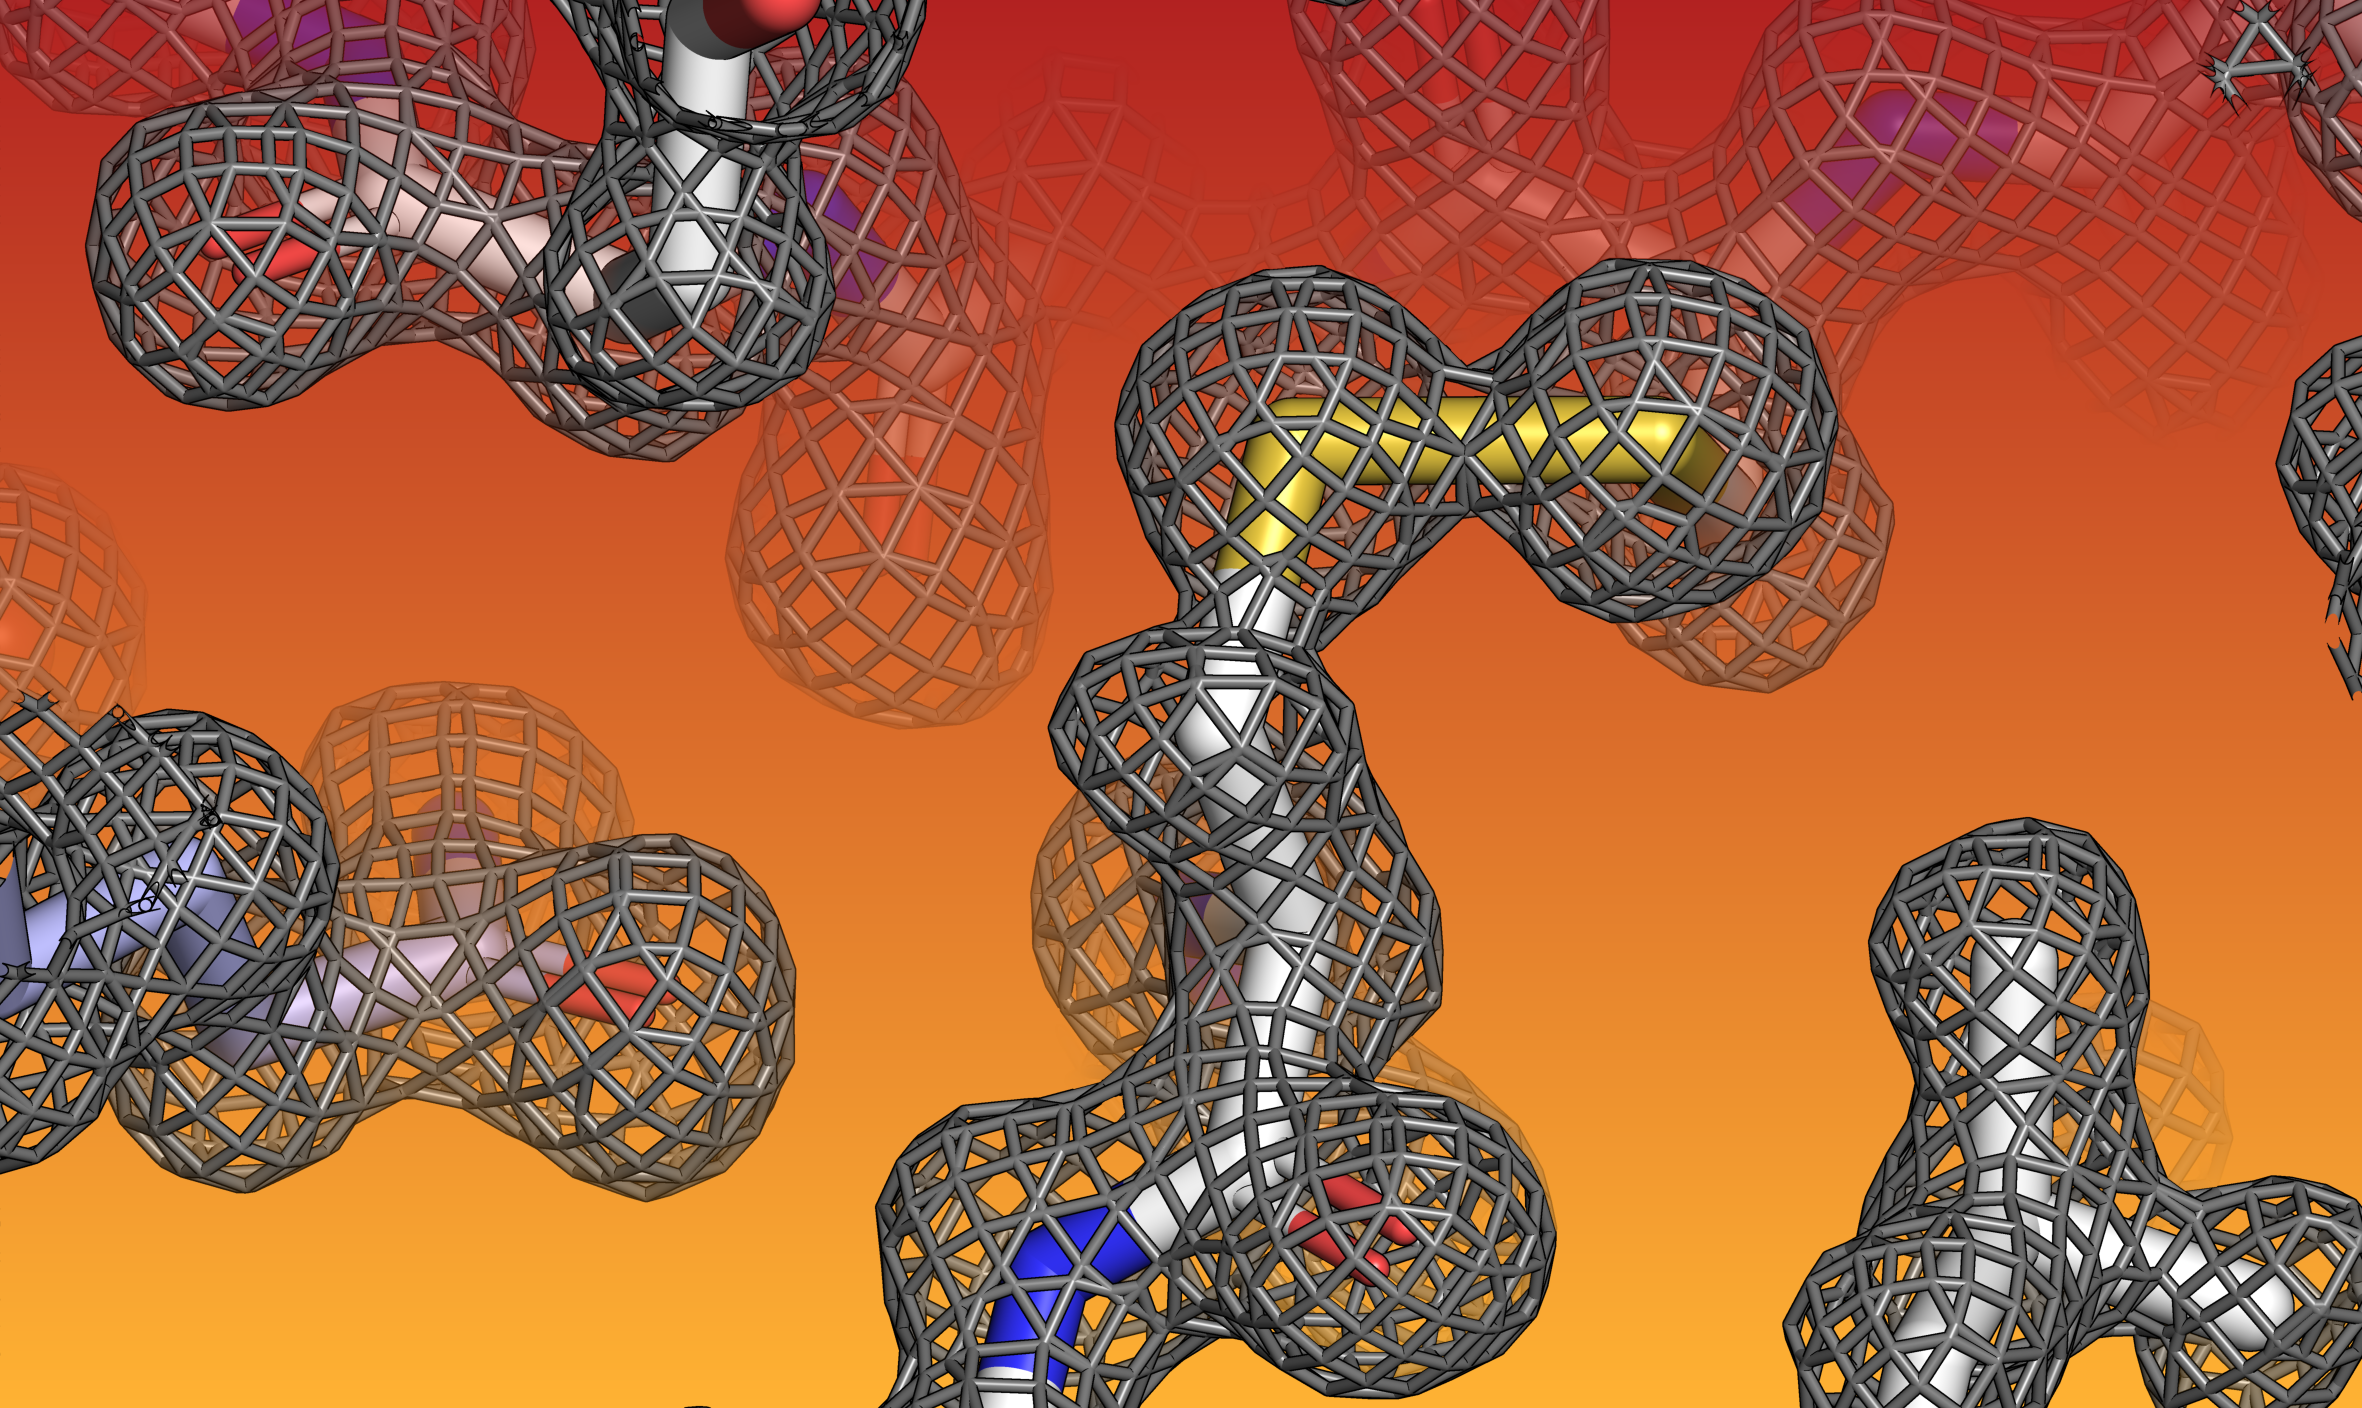
\includegraphics[width=0.8\textwidth]{after.png}
    \caption{Lisozima, colecta 2 a \SI{3.2}{\mega\gray}. Datos de \cite{Nanao2005}.}
  \end{figure}
\end{frame}
%----------------------------------------------------------------------------------------
\begin{frame}{Consecuencias: daño específico}
%El daño por radiación sobre ciertos residuos de aminoácido. No ocurre de manera idéntica. Modelo estructural \emph{perturbado}.
\begin{figure}[h]
	\centering
	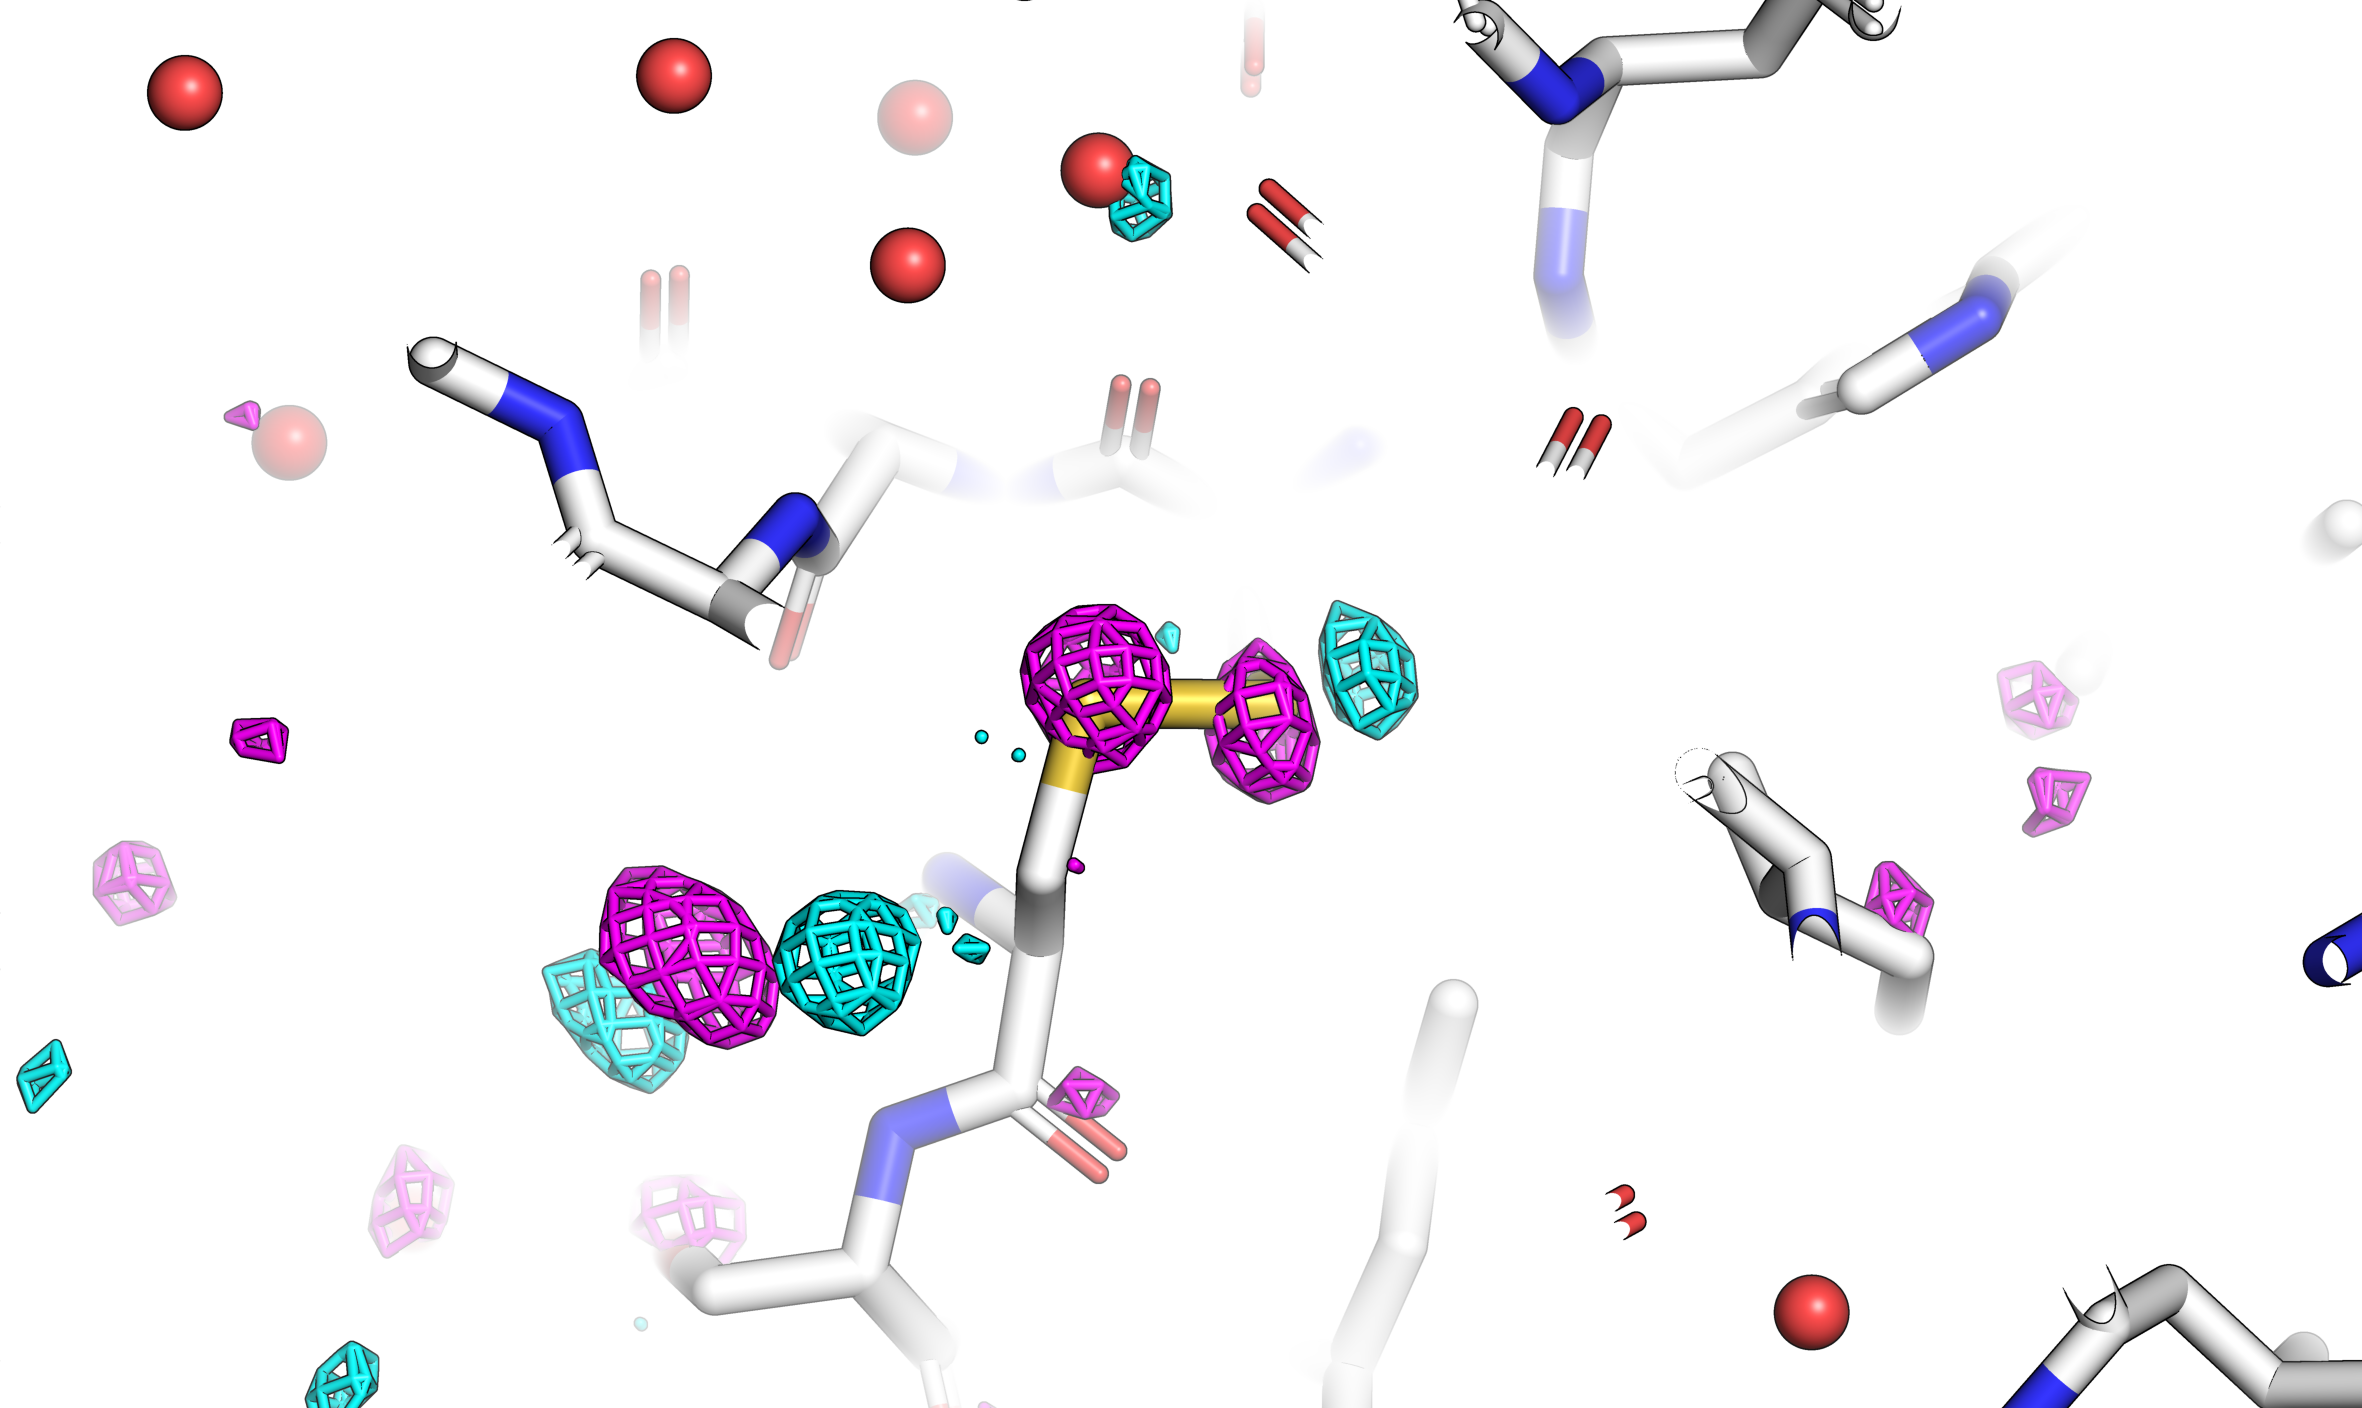
\includegraphics[width=0.8\textwidth]{diff.png}
	\caption{Diferencia de densidad electrónica entre colectas de datos. }
	\label{fig:nanao2005}
\end{figure}
\end{frame}
%----------------------------------------------------------------------------------------
\begin{frame}{Consecuencias: daño global}
\label{teng}	
La pérdida de reflexiones y su disminución en intensidad en los patrones de difracción. 
\begin{figure}[h]
  \centering
  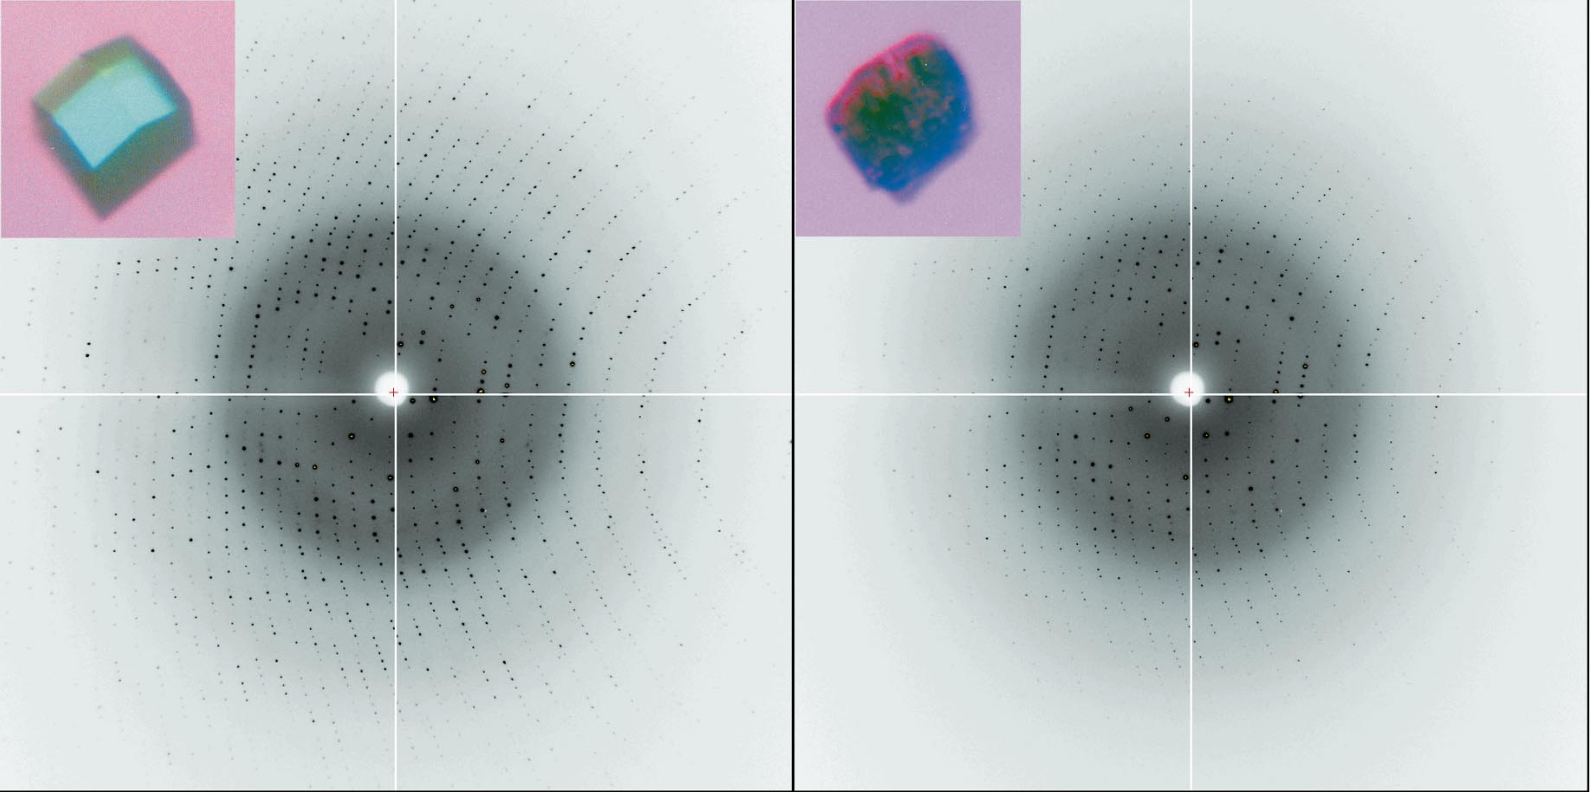
\includegraphics[width=0.8\textwidth]{teng.png}
  \caption{Cristal de lisozima y su patrón de difracción después de una dosis de radiación de \SI{120}{\kilo\gray} (izquierda) y \SI{16.7}{\mega\gray} (derecha). Fuente: \cite{Teng2000}. Información sobre \hyperlink{backup:grays}{\beamergotobutton{Grays}}. }
  \label{fig:teng2000}
\end{figure}
\end{frame}
%----------------------------------------------------------------------------------------
\begin{frame}{Consecuencias: daño global}
Después de procesar los patrones de difracción, el daño por radiación se nota en:
\begin{itemize}
  \item Cambio del volumen de la celda unitaria
  \item Aumento del factor de escala
  \item Deterioro de las métricas que evalúan la calidad de los datos y la relación entre datos y el modelo estructural. 
\end{itemize}
\end{frame}
%----------------------------------------------------------------------------------------
\begin{frame}{Consecuencias: peor escenario}
	\begin{alertblock}{Nada}
		En el peor de los casos, es imposible obtener un modelo estructural.
	\end{alertblock}
\end{frame}
%----------------------------------------------------------------------------------------
\begin{frame}{Radioprotectores}
Interacción con los radicales libres antes que la proteína.
\begin{figure}[h]
	\centering
	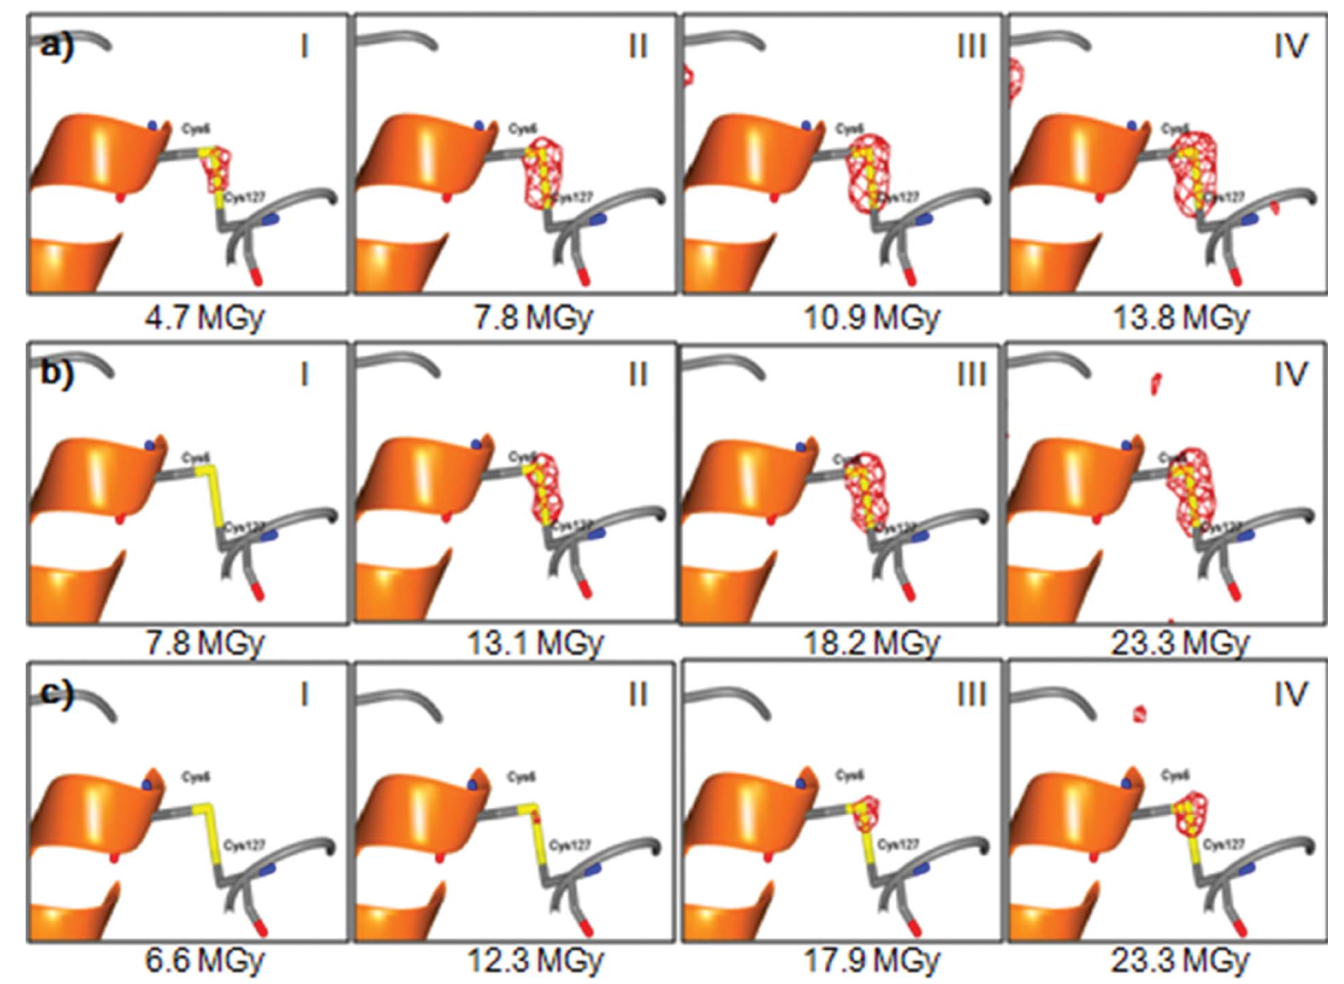
\includegraphics[width=0.7\textwidth]{delamora2011.png}
	\caption{Radioprotectores en cristal de lisozima nativo (a), con ácido ascórbico (b) y con nitrato de sodio (c). Imagen tomada de \cite{DeLaMora2011}.}
	\label{fig:delamora2011}
\end{figure}
\end{frame}
%----------------------------------------------------------------------------------------
\begin{frame}{To scavenge or not to scavenge}
En comparación con la crioprotección, el uso de radioprotectores todavía no se ha adoptado como parte de la rutina de la CRX \cite{Nowak2009,Allan2013}. Además de algunas incertidumbres experimentales\footnote{Parámetros necesarios en la estimación de la dosis.}, esto se debe a:
\begin{itemize}
  \item Los cristales pueden ser muy diferentes.
  \item Uso de diferentes métricas.
  \item Complejidad de la condición de cristalización.
\end{itemize}
\end{frame}
%----------------------------------------------------------------------------------------
%	 ANTECEDENTES
%----------------------------------------------------------------------------------------
\section{Antecedentes}
%----------------------------------------------------------------------------------------
\begin{frame}{pH}
El electrón solvatado se encuentra en un equilibrio ácido base:
\begin{equation*}
\ce{e^{-}_{solv.} + H^{+} <=> H^{.}}
\end{equation*}
El radical \ce{H^.} se puede recombinar:
\begin{equation*}
   \ce{2H^{.}      ->        H2}
\end{equation*} 
Se ha probado que el \ce{H2} es uno de los principales productos de la radiación \cite{Meents2010}. 
%En este caso el ion oxidanio funciona como radioprotector. 
\end{frame}
%----------------------------------------------------------------------------------------
\begin{frame}{pH}
En mi tesis de maestría se investigó el efecto del pH sobre el daño específico en los puentes disulfuro, en cristales de lisozima: el cristal con el pH más ácido (3.7) presentó mayor daño por radiación que el cristal con el pH más básico (5.7).
\end{frame}
%----------------------------------------------------------------------------------------
%	 OBJETIVOS
%----------------------------------------------------------------------------------------
\section{Objetivos}
%----------------------------------------------------------------------------------------
\begin{frame}{Objetivos}
	Determinar el efecto del pH sobre el daño por radiación.
\begin{enumerate}
	\item Hallar una lista de proteínas capaces de cristalizar en un intervalo de pH \emph{amplio}
	\item Cristalizarlas
	\item Difractarlas
	\item Obtener las estructuras 
	\item Realizar un análisis con mapas de diferencia de densidad electrónica
\end{enumerate}	
\end{frame}
%----------------------------------------------------------------------------------------
%	 MATERIALES Y MÉTODOS
%----------------------------------------------------------------------------------------
\section{Materiales y métodos}
%----------------------------------------------------------------------------------------
\begin{frame}{Lista de proteínas}
Para obtener la lista de proteínas, se usó la información del banco de datos de proteínas (\href{https://www.rcsb.org/}{PDB}, por sus siglas en inglés).
  \begin{enumerate}
    \item Descarga el PDB completo (formato \texttt{.mmcif})
    \item Extrae información del cabezal
    \item Aplica filtros (\texttt{R} y \texttt{bash})
    \begin{itemize}
      \item Si no tiene una anotación del pH
      \item Resolución útil (menor a \SI{2}{\angstrom})
      \item Número de entidades igual a 1
      \item Secuencia similar a la secuencia consenso
      \item Cristalice en un intervalo de pH amplio
    \end{itemize}
  \end{enumerate}
\end{frame}
%----------------------------------------------------------------------------------------
\begin{frame}{}
 \begin{figure}
   \centering
   \includegraphics[width=0.7\textwidth]{}
   \caption{Alineamiento múltiple con MAFFT \cite{Katoh2012}}
 \end{figure} 
\end{frame}
%----------------------------------------------------------------------------------------
\begin{frame}{}
  
\end{frame}
%----------------------------------------------------------------------------------------
\begin{frame}{Colecta de datos}
	Para los cristales de cada proteína se realizaran colectas idénticas de manera repetitiva hasta alcanzar el límite de dosis absorbida permitida (\SI{30}{\mega\gray}).
\end{frame}
%----------------------------------------------------------------------------------------
\begin{frame}{Procesamiento de datos}
Se resolveran las estructuras por reemplazo molecular y se crearan mapas de diferencia de densidad electrónica para analizar la diferencia en daño por radiación a distintos pHs tratando de mantener un nivel de dosis absorbida comparable.
\end{frame}
%----------------------------------------------------------------------------------------


%----------------------------------------------------------------------------------------
%	 DISCUSIÓN
%----------------------------------------------------------------------------------------
\section{Discusión}
%----------------------------------------------------------------------------------------
\begin{frame}{}
	.... y ya.
\end{frame}
%----------------------------------------------------------------------------------------
\begin{frame}{Título x}
	Algo de texto por aquí y por allá.
\end{frame}
%----------------------------------------------------------------------------------------
\begin{frame}{Título x}
	Algo de texto por aquí y por allá.
\end{frame}
%----------------------------------------------------------------------------------------
%	 CONCLUSIÓN
%----------------------------------------------------------------------------------------
\section{Conclusión}
%----------------------------------------------------------------------------------------
\begin{frame}{Título x}
	Algo de texto por aquí y por allá.
\end{frame}
%----------------------------------------------------------------------------------------
%	 CLOSING/SUPPLEMENTARY SLIDES
%----------------------------------------------------------------------------------------
\appendix
%----------------------------------------------------------------------------------------
\begin{frame}{Grays}
\label{backup:grays}
Un Gray (\si{\gray}) según el Sistema Internacional de Unidades, es un Joule (\si{\joule}) de energía absorbida por kilogramo (\si{\kilogram}) de materia.
Contexto:
\begin{table}[]
  \centering
  \begin{tabular}{lr}
  \toprule
  Especie & $\mathrm{LD}_{50/30}$ (\si{\gray})\\
  \midrule
  Humano & $\sim$2.5-4.5 \\
  Mono & 4.5 \\
  Ratón & 4.5 \\
  Rata & 6.0 \\
  Pez dorado & 7.5 \\
  Conejo & 8.0 \\
  Cucaracha & 50.0 \\
  \bottomrule
	\end{tabular}%
	\caption{Dosis letal para el \SI{50}{\percent} de la población después de 30 días para diferentes especies. Cuadro modificado de \cite{Bolus2017}. \hyperlink{teng}{\beamerreturnbutton{Regresa}}} 
	\label{tab:LD5030}
\end{table}
\end{frame}
%----------------------------------------------------------------------------------------
\begin{frame}[allowframebreaks]{Referencias}
	%\nocite{*} % Display all references regardless of if they were cited
	\bibliography{bib.bib}
	\bibliographystyle{unsrt}
\end{frame}
%----------------------------------------------------------------------------------------
\end{document}
%----------------------------------------------------------------------------------------
